\documentclass[12pt,a4paper]{ctexart}
\usepackage{geometry}
\geometry{left=2.5cm,right=2.5cm,top=2.0cm,bottom=2.5cm}
% \usepackage[english]{babel}
\usepackage{amsmath,amsthm}
\usepackage{amsfonts}
\usepackage[longend,ruled,linesnumbered]{algorithm2e}
\usepackage{fancyhdr}
\usepackage{array}
\usepackage{listings}
\usepackage{color}
\usepackage{graphicx}
\usepackage{minted}
\usepackage{float}
\usepackage[defaultmono]{droidsansmono}

\graphicspath{{pics/}}
\ctexset{today=small}
\definecolor{codebg}{rgb}{0.95,0.95,0.95}

\input{personal_info/info.tex}

\begin{document}
    \begin{titlepage}
        \heiti
        \vspace*{64pt}
        \begin{center}
            \fontsize{48pt}{0} 算法设计与分析\\
            \vspace*{36pt}
            \fontsize{48pt}{0}{实\quad 验\quad 报\quad 告}\\
            \vspace*{48pt}
            \LARGE(2021\~{}2022 学年度\qquad 第 3 学期)\\
            \vspace*{48pt}
        
            \LARGE 实验名称\ \ \underline{\makebox[200pt]{\ExamTitle}}\\
            \LARGE 实验地点\ \ \underline{\makebox[200pt]{\ExamAddr}}\\
            \LARGE 实验日期\ \ \underline{\makebox[200pt]{\today}}\\
            \LARGE 学生姓名\ \ \underline{\makebox[200pt]{\MyName}}\\
            \LARGE 学生学号\ \ \underline{\makebox[200pt]{\MySID}}\\
            \LARGE 指导教师\ \ \underline{\makebox[200pt]{\TeacherName}}\\
            \vspace*{48pt}
            
            \LARGE 东南大学\quad  计软智学院 \quad 制
        \end{center}
    \end{titlepage}

\title{
  {\heiti \textbf{实验六\ 贪心算法}
    \footnote{要求:1、分析题请用书面化语言给出详细分析过程。2、实验请统一使用ex0*-学号-姓名的命名格式,latex版本请附上源代码并打包提交。}
    }
}
\date{}

\maketitle

\section*{\bf \color{black}{一、实验目的及意义}}
\noindent
\begin{enumerate}
	\item[(1)]  掌握贪心算法的基本思想、求解问题的基本步骤;
	\item[(2)]  学会利用贪心算法解决实际问题。
\end{enumerate}

\vspace{5pt}

\section*{二、实验内容与结果}
\subsection*{题目1:药品放置问题}
\paragraph{题目内容}
\subparagraph{题目描述}
\begin{itemize}
    \item 有多个药品要放入多个房间,每个药品放入房间时,均有一个放入时间s和取出时间f(s、f为大于等于0的整数,s小于f),以及该物品的特性c(c取值为7、8、9、10、11、12中的一个)。
    \item 两个药品若同时满足以下2个条件时,则它们不能被放在同一个房间:
    \item 1)两个药品在放入时间和取出时间上有重叠,比如药品1的s、f分别取3、10,药品2的s、f分别取9、15;
    \item 2)药品1的特性值c1,与药品2的特性值c2相同;若上述2个条件至少有一个不满足,则这2个药品可以放在同一个房间。
\end{itemize}

问:给定n个药品的s、f、c参数,以及k个房间,问这k个房间最多可以放下多少种药品?

\subparagraph{输入格式}
    \begin{itemize}
        \item 第一行输入一个整数n和k,分别表示药品种数,以及房间个数。
        \item 紧接着n行,每一行3个数字s、f、c,以空格隔开,分别表示对应药品的放入时间、取出时间、药品特性。
    \end{itemize}
\subparagraph{输出格式}
    \begin{itemize}
        \item 一个整数,表示这k个房间最多可以放下的药品种数。
    \end{itemize}

\subparagraph{输入输出样例}
如下表
    \begin{figure}[h]
        \centering
        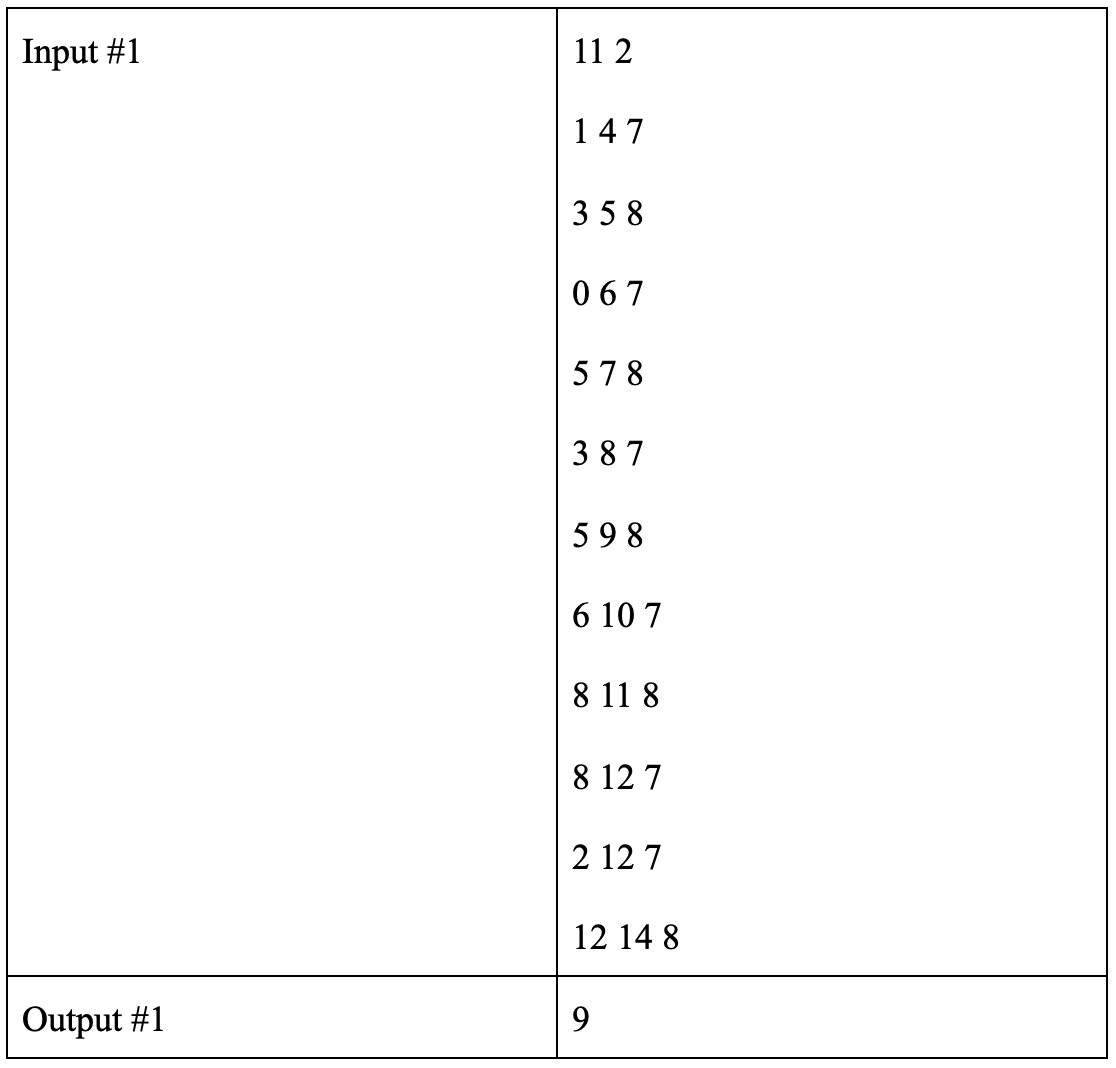
\includegraphics[width=0.80\textwidth]{q1_iodata.png}
    \end{figure}

\vspace{5pt}

\paragraph{实验环境}
\begin{itemize}
    \item 程序设计语言:C++
    \item 编程环境:
    \begin{itemize}
        \item 编辑器:Visual Studio Code (1.67.0)
        \item 编译器:g++ (GCC) 11.2.0
        \item 操作系统:ArchLinux 5.17.5-zen1-1-zen (64-bit)
    \end{itemize}
\end{itemize}

\vspace{5pt}

\paragraph{解答} 本题未完成

源码:
\inputminted[bgcolor=codebg,frame=lines,autogobble,linenos=true,breaklines]{cpp}{src/t1.cpp}

\vspace{5pt}

\paragraph{实验结果}
本题未完成

\newpage

\subsection*{题目2:最优特征子序列}
\paragraph{题目内容}
\subparagraph{题目描述}
\begin{itemize}
    \item 给定字符串 s, 其特征子序列 t 满足:
    \item 1) 子序列中的字符各不相同;
    \item 2) s中的各种字符都能在 t 中找到;
    \item 对于一个字符串 s,可能会对应多个特征子序列,其中字典序最小的特征序列称为“最优特征子序列”。
    \item 请写一个程序,返回字符串的最优特征子序列。要求时间复杂度不超过O(N)。
\end{itemize}

\subparagraph{输入格式}
    \begin{itemize}
        \item 第一行输入长度 N;
        \item 第二行输入长度为 N 的字符串 s.

    \end{itemize}

\subparagraph{输出格式}
    \begin{itemize}
        \item 返回最优特征子序列。
    \end{itemize}
    
\subparagraph{输入输出样例}
如下表
    \begin{figure}[h]
        \centering
        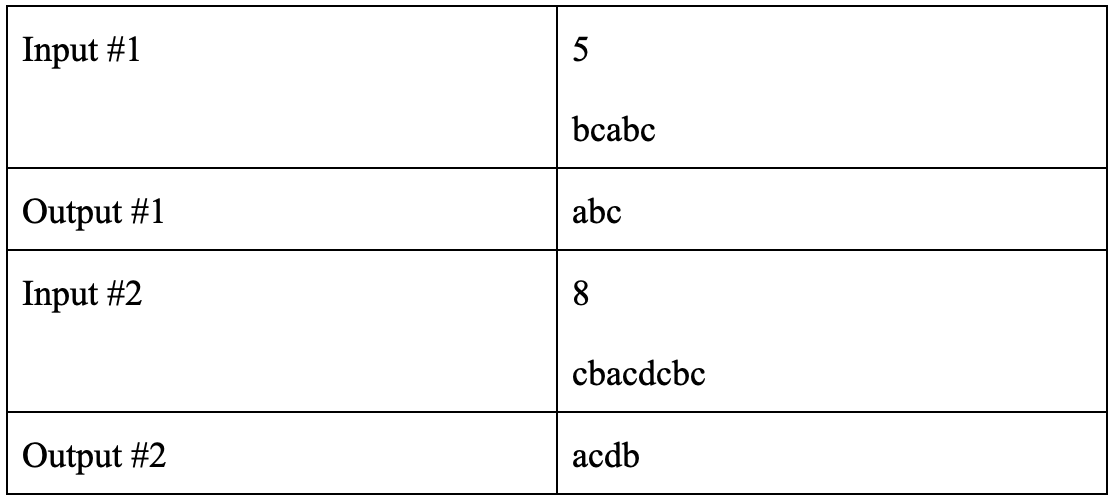
\includegraphics[width=0.80\textwidth]{q2_iodata.png}
    \end{figure}


\vspace{5pt}

\paragraph{实验环境}
\begin{itemize}
    \item 程序设计语言:C++
    \item 编程环境:
    \begin{itemize}
        \item 编辑器:Visual Studio Code (1.67.0)
        \item 编译器:g++ (GCC) 11.2.0
        \item 操作系统:ArchLinux 5.17.5-zen1-1-zen (64-bit)
    \end{itemize}
\end{itemize}

\vspace{5pt}

\paragraph{解答} 本题未完成

源码:
\inputminted[bgcolor=codebg,frame=lines,autogobble,linenos=true,breaklines]{cpp}{src/t2.cpp}

\vspace{5pt}

\paragraph{实验结果}
本题未完成

\newpage

\subsection*{题目3:移动筹码}
\paragraph{题目内容}
\subparagraph{题目描述}

\begin{itemize}
    \item 数轴上放置了一些筹码,每个筹码的位置存放在数组 chips 当中。你可以对任何筹码 执行下面两种操作之一(不限操作次数,0 次也可以):
    \item 将第 i 个筹码向左或者右移动 2 个单位,代价为 0。
    \item 将第 i 个筹码向左或者右移动 1 个单位,代价为 1。
    \item 最开始的时候,同一位置上也可能放着两个或者更多的筹码。返回将所有筹码移动到同一位置(任意位置)上所需要的最小代价。

\end{itemize}

\subparagraph{输入格式}
    \begin{itemize}
        \item 第一行输入筹码个数 N;
        \item 第二行输入长度为N的数组,表示每个筹码所在位置。
    \end{itemize}

\subparagraph{输出格式}
    \begin{itemize}
        \item 输出移动筹码的最小代价。
    \end{itemize}
    

\subparagraph{输入输出样例}
如下表
    \begin{figure}[h]
        \centering
        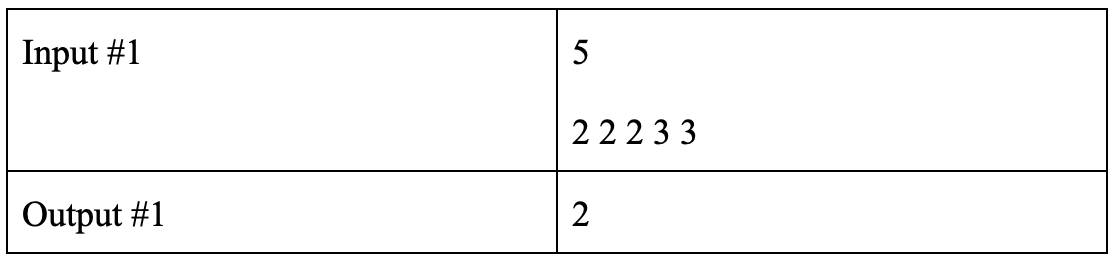
\includegraphics[width=0.80\textwidth]{q3_iodata.png}
    \end{figure}

\vspace{5pt}

\paragraph{实验环境}
\begin{itemize}
    \item 程序设计语言:C++
    \item 编程环境:
    \begin{itemize}
        \item 编辑器:Visual Studio Code (1.67.0)
        \item 编译器:g++ (GCC) 11.2.0
        \item 操作系统:ArchLinux 5.17.5-zen1-1-zen (64-bit)
    \end{itemize}
\end{itemize}

\vspace{5pt}

\paragraph{解答} 时间复杂度:$O(N)$

源码:
\inputminted[bgcolor=codebg,frame=lines,autogobble,linenos=true,breaklines]{cpp}{src/t3.cpp}

\vspace{5pt}

\paragraph{实验结果}
(可附上截图)

\newpage

\section*{三、心得体会}
    可根据“实验思考”部分作答,也可以根据个人具体体会作答。自己算法的创新点可在此处进行介绍,酌情加分。

\end{document} 
